\chapter{Wideband Cognitive Spectrum Sensing}\label{C:wideband_css}

Cognitive Radio (CR) has been attracting many attention in recent researches with respect to the potential better utilisation performance of limited spectrum resources. In this chapter, we first propose an overview of cognitive radio networks. Then we focus on the bottleneck in its front-end sampling devices and investigate the typical CS framework for spectrum sensing in CR. 

\section{Introduction}

As the wireless techniques keep fast developing, the limited spectrum resource seriously restricts the fast increasing demand for more accessible bandwidth. As a result, the dynamic spectrum access (DSA) becomes necessary and popular, which enables unused spectrum accessed opportunistically, shown in figure \ref{dsa-cr-intro}.(a). 

Following this idea, the cognitive radio (CR) develops aiming at optimizing utilisation of idle bands for communications, without doing harm to the primary users (licensed spectrum) \cite{akyildiz2006next}. Correspondingly, the CR devices have to sense the environment (including spectrum usage, noise level etc) quickly and accurately, and reconfigure themselves to adapt the varying circumstance.

\begin{figure}
\centering
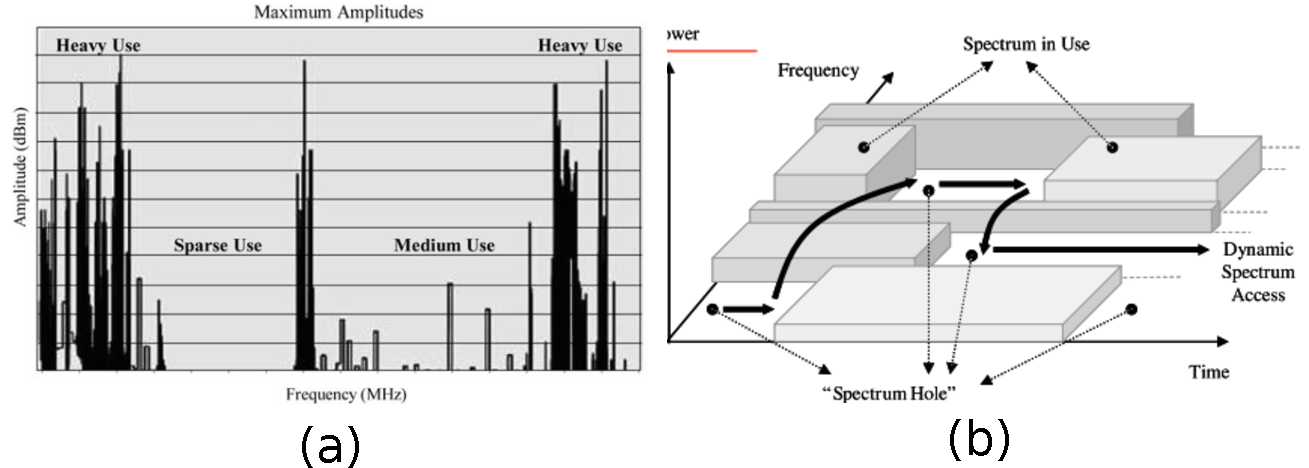
\includegraphics[width=0.85\columnwidth]{figs/cr-intro.pdf}
\caption{(a) The existence of unused spectrum resources; (b) The concept of spectrum holes}
\label{dsa-cr-intro}
\end{figure}

Therefore, in cognitive radios, the first and important procedure is to sense the unused bandwidth, termed as the spectrum holes and shown in figure \ref{dsa-cr-intro}.(b). If the band is detected as unused, the CR networks will use it for further communication. Otherwise, the CR moves to find other spectrum holes, or stays in the same band but avoid interference by changing its transmission power or modulation model.

However, trends of communicating requires higher frequency and wider bandwidth. As a result, signal acquisition significant is crucial according to the Nyquist sampling theory. What's worse, since CR should not generates additional interference to the licensed users, CR must limits its working power to a relatively low level (if CR do not change its modulation model). The demand for sensing with low power contradicts with the requirement for sensing in high sensitivity. Thus this contradiction makes the signal acquisition much more difficult. 

In conclusion, spectrum sensing becomes one of the most crucial problem for cognitive radios, and it is still an open issue. Then, compressed sensing will be introduced to be embedded into traditional spectrum sensing algorithms, in order to solve the problem and enhance the overall performance.

\section{Spectrum Sensing}\label{sct:ssm}

%re-wr:
A cognitive radio supports the capability to select the best available channel \cite{akyildiz2006next}, and the main functions for cognitive radios in xG networks can be summarized as \cite{haykin2005cognitive}, where the spectrum sensing to decide whether a particular sub-band of the spectrum is available or not, without harmful interference with primary users. It is the first procedure in cognitive radio networks where various parameters are detected for further spectrum management, spectrum mobility and spectrum sharing. 

%\begin{itemize}
%\item{Spectrum sensing:} detecting unused spectrum without harmful interference to primary users.
%\item{Spectrum management:} capturing the best available spectrum to meet user communication requirements.
%\item{Spectrum mobility:} maintaining seamless communication requirements during the transition to better spectrum.
%\item{Spectrum sharing:} providing the fair spectrum scheduling method among second users.
%\end{itemize}

\subsection{Aim: Spectrum Usage Detection}\label{sct:aim_ss}

According to the aim of spectrum sensing, the main task becomes to decide whether a particular sub-band of the spectrum is available or not, namely, to detect spectrum usage situation. A widely accepted idea is to detect the signal existence from licensed users' (primary users, PUs) communication at cognitive radio's receivers: if the PU's signal (in the particular sub-band) are not detected, cognitive radios can access the band for further communication; otherwise, CR cannot use the band. 

\subsection{Hypothesis Detection Model}

In this subsection, the problem of detecting the signal existence from PUs is modelled by two hypotheses in equation \ref{detect_hypo}: 
\begin{equation}
\label{detect_hypo}
\begin{aligned}
H0: y[n] = w[n]   \\
H1: y[n] = w[n] + x[n] 
\end{aligned}
\end{equation}
, where $x[n]$ is the primary user's signal, $y[n]$ is the vectorial observation, $w[n]$ is the noise, and $n$ refers to time slots. The hypothesis 1 suggests that the primary user's signal exists, while hypothesis 0 suggests no. Typically, the decision is made by comparing a predetermined threshold with test statistic $\Lambda(y)$ in equation \ref{detect_statistic}: 
\begin{equation}
\label{detect_statistic}
\Lambda(y) \mathop{\lessgtr}_{H_1}^{H_0} \alpha
\end{equation}
Then the performance of a detector is quantified by the receiver operating characteristics (ROC) curve, which presents the probability of detection $P_D = Prob(\Lambda(y) > \alpha, H1)$ and false alarm probability $P_fa = Prob(\Lambda(y) > \alpha, H0)$. 

\section{Traditional Detection Method}

\subsection{Narrowband Detection}

In this section, typical spectrum sensing approaches are introduced. Narrowband sensing algorithms can be suitably applied when the channel frequency response is flat. The following figure \ref{narr_spec_sens} demonstrates most typical architectures in narrowband spectrum sensing.

\begin{figure}
\centering
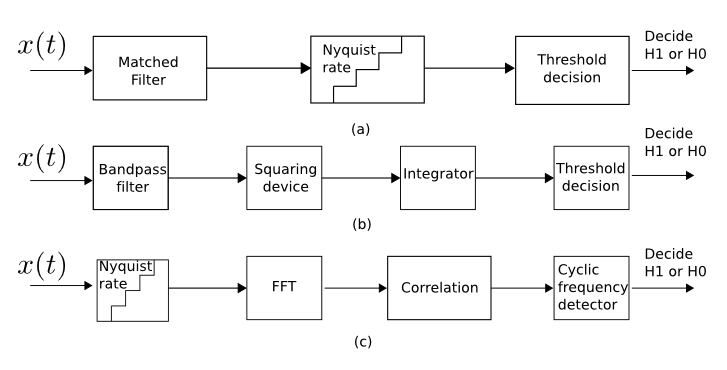
\includegraphics[width=0.75\columnwidth]{figs/narr_spec_sens.png}
\caption{Block diagrams for traditional narrowband detection architectures: $a)$ matched filtering detector; $b)$ energy detector; $c)$ feature detector}
\label{narr_spec_sens}
\end{figure}

\subsubsection{Matched filter}
In the figure \ref{narr_spec_sens}.(a), the matched filtering (MF) detector\cite{poor1994introduction} is presented. when the signal to be detected is perfectly known (i.e. mean and variance), the optimal test statistic is produced by matched filter by correlating the received signal to a template. However, the signal cannot always be known in practise, so sometimes it's not applicable. Besides, the carrier synchronisation is also a remained difficult problem.

\subsubsection{Energy detector}
In the figure \ref{narr_spec_sens}.(b), the energy detector (ED) \cite{urkowitz1967energy} is presented. In the case where the signal to be detected does not present structure template, the ED can produce the optimal test statistic by directly analysis the power and variance of the received signal. The implementation of ED is simple, but it suffers from poor detection results in low SNR environment. Besides, the ED cannot distinguish different primary signals at the same time.

\subsubsection{Feature detector}
In the figure \ref{narr_spec_sens}.(c), cycle-stationary feature detection (FD) \cite{enserink1994cyclostationary} is presented. If discrimination for primary signals and higher detection performance are required, the FD exploits the cyclic non-stationary features from primary signals. The cyclic features can be found in many typical modulated signals, for instance, in the orthogonal frequency-division multiplexing (OFDM) contains cyclic features in correlation structure due to the cyclic prefix (CP) between transmitted data. However, the computational cost is relatively high and long running time delay is always existing. 

\subsection{Nyquist Wideband Detection}\label{sct:wss}

In the scenarios where the bandwidth is sufficiently larger than coherence bandwidth of channel, wideband sensing is more suitable than narrowband sensing. For instance, it can be used for sensing the ultra-high-frequency (UHF) TV band, ranging from 300 MHz to 3 GHz, while the narrowband sensing providing single binary decision over whole spectrum is always not suitable for identifying individual spectrum access opportunities. The following figure \ref{nqys_spec_sens} demonstrates the typical architectures for wideband spectrum sensing and detection.

\begin{figure}
\centering
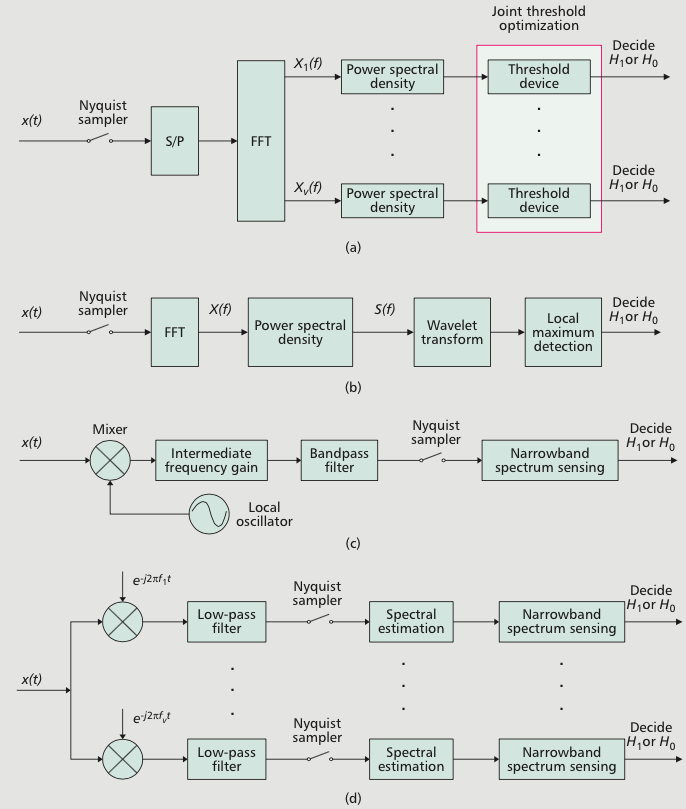
\includegraphics[width=0.75\columnwidth]{nqys_spec_sens.png}
\caption{Block diagrams for Nyquist wideband detectors architectures: $a)$ multiband joint detector; $b)$ wavelet detector; $c)$ sweep-tune detector; $d)$ filter-bank detector}
\label{nqys_spec_sens}
\end{figure} 

\subsubsection{Multiband joint detector}
In figure \ref{nqys_spec_sens}.(a), the multiband joint detector (MJD) \cite{quan2009optimal} is presented. The MJD first uses serial-to-parallel conversion (S/P) to divide samples into parallel data streams, then it process the FFT to divide spectrum X(f) into groups of narrowband spectrum. Then each binary hypothesis detection is performed and joint optimised at last. The high sampling rate and lower speed of joint optimisation is the main bottleneck.

\subsubsection{Wavelet detector}
In figure \ref{nqys_spec_sens}.(b), the wavelet detector\cite{tian2006wavelet} is introduced. The wavelet analysis of power spectral density (PSD) can provide significant border symbols of two neighbour sub-bands, the aim of detection becomes a spectral edge detection problem. However, the high sampling rate is also the bottleneck.

\subsubsection{Sweep-tune detector}
In figure \ref{nqys_spec_sens}.(c), the sweep-tune detector\cite{quan2009optimal, farhang2008filter} is displayed. This detector uses a special frequency mixing technique that 'sweep' across the frequency range of interest, to down-converts signals to a lower frequency. The adaptive local oscillator (LO) is used for 'sweep' procedure. However, the procedure of 'sweep' mixing generates too much time to wait.

\subsubsection{Filter-bank detector}
Also using the idea of down-conversion, the figure \ref{nqys_spec_sens}.(d) shows the structure of filter-bank detector \cite{farhang2008filter}. Not only following the technique which 'sweep' mixing the interest of signals, it also applies parallel structure to speed up the processing time by using filter-bank. As a result, the time cost of mixing reduces but the implementation cost largely increase.

\section{Sub-Nyquist Wideband Detection}

Different from Nyquist wideband detection, the sub-Nyquist spectrum sensing applies the multi-coset (MC) sampling, multi-rate (MR) sampling, or compressed sensing (CS) to reduce the required sampling rate. Before talking about CS based sampling, first we take brief look at MC and MR sampling.

\subsubsection{Multi-Coset Sampling}

The multi-coset (MC) sampling \cite{venkataramani2000perfect} applies blocks of parallel consecutive samples with special time offsets to sample, so that each channel has a task of low-rate sampling. Then joint spectrum recovery and further detection can be performed. The main difficulty is how to perform sampling channel synchronisation with highly accurate time offsets. The quality of the specific offsets is crucial for robustness in its spectral reconstruction.

\subsubsection{Multi-Rate Sampling}

The multi-rate (MR) sampling \cite{sun2013wideband} uses various sampling rates to wrap different sparse spectrum onto individual channels, and then use joint sparse spectrum recovery for further energy detection. Time synchronisation is no longer needed compared to the MC. But instead, the sacrifice is the hardware cost for parallel structure, as well as the increased sampling rate compared to original CS although the MR's sampling rate is still less than Nyquist rate. 

\section{CS based Detection Method}\label{sct:cwd}

\subsection{Introduction to Compressive Spectrum Sensing }\label{sct:css}

Cognitive spectrum sensing is another typical application suitable for compressed sensing. The applicability of Compressive spectrum sensing (CSS )mainly lies in two aspects:  

\paragraph{Sampling Rate}
The trend of higher frequency transmission is also suitable for cognitive radio, which leads to higher rate sampling rate at receivers. Thus it's reasonable to develop the CS based spectrum sensing techniques to reduce the sampling rate.

\paragraph{Flexibility and Energy}
The cognitive radio requires flexibility for sensing various  types of signals (TV signal, cell phone, satellites etc) in a relatively wide bandwidth. However, normal wideband spectrum detection uses filtering or mixing for down-conversion (then low-rate sampling). This approach require difficult analog implementations such as adaptive local oscillator(LO) for filter-banks(FB). Inversely, if the CS is used, then the system can get wider sensing (frequency) ranges without the hardware of LO or FB.

Therefore, the CS become popular in cognitive spectrum sensing. The figure \ref{comp_spec_sens} demonstrates the typical architectures in wideband spectrum sensing, and briefly analyse CS detectors. The similar CS based architecture can also be viewed in chapter \ref{C:compressed_sensing}.

\subsection{Compressive Detectors Overview}
\begin{figure}
\centering
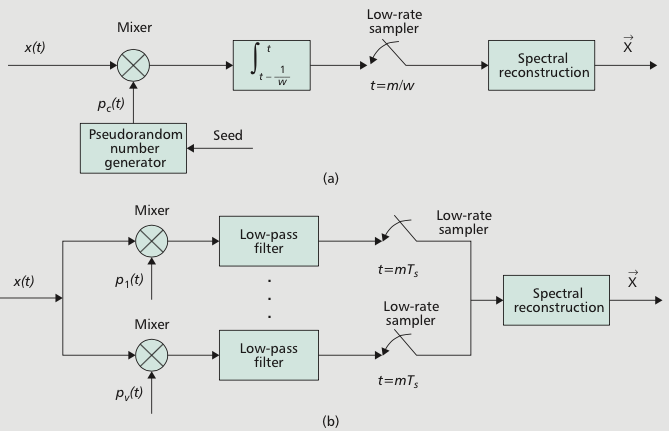
\includegraphics[width=0.75\columnwidth]{figs/comp_spec_sens.png}
\caption{Block diagrams for compressive wideband sensing architectures: $a)$ random demodulation based detector; $b)$ modulated wideband converter-based detector}
\label{comp_spec_sens}
\end{figure} 

\subsubsection{Demodulation based Detector}  
Figure \ref{comp_spec_sens}.(a) presents the random demodulation (RD) based detector\cite{tropp2010beyond}, which is an analog-to-information converter (AIC) for finite-length and discrete-time signals, and consists of pseudorandom wave generator, a mixer, and a low-rate ADC. The detailed architecture of RD is introduced in chapter \ref{C:compressed_sensing}. The reconstruction of RD sampled data involves $l1$-norm minimization (e.g. based BP, LASSO) or greedy method (e.g. OMP).
This design is simple, but easily affected by model mismatches and design imperfections.

\subsubsection{Modulated Wideband Converter based Detector}
Figure \ref{comp_spec_sens}.(b) displays the modulated wideband converter (MWC) based detector \cite{mishali2009expected} for the case where multichannel signals are designed to be detected. The MWC can be considered as a parallel structure of RD, and its architecture is introduced in chapter \ref{C:compressed_sensing}. The reconstruction of MWC involves the multiple measurement vector (MMV) sparse recovery which exploits the fact that the columns of original spectrum coefficients share the same sparsity pattern. Compared to the RD, MWC provides robustness against the noise and model mismatches.

\subsubsection{Cooperative Compressive Spectrum Sensing} 
%re-write{
Cooperative versions of spectrum sensing is an open issue, which aims at solving the hidden terminal problem \cite{akyildiz2006next} and improve sensing accuracy. The cooperative version of compressive wideband sensing have
 been developed \cite{tian2008compressed, wang2009distributed}. Here, individual radios can make a local decision about the presence or absence of a primary user, and these results can then be fused in a centralised or decentralised manner. However, a greater cooperation gain can be achieved by fusing all the compressed measurements, again in a centralised or decentralised manner. In general, such measurement fusion requires that each cognitive radio knows the channel state information (CSI) from all primary users to itself \cite{tian2008compressed}, which is cumbersome. But recent extensions show that measurement fusion can also be carried out without CSI knowledge \cite{fanzi2011distributed}.
%}

\subsection{An Instance: CS based Cognitive Radar System}
In \cite{stinco2014compressed} the CS is embedded to enhance the performance of cognitive radar that use wide operating frequency bandwidths for spectrum sensing and sharing. The compressive cognitive radar  utilises the typical CS techniques, including the random demodulation (RD) for signal acquiring, basis pursuit de-noising (BPDN) algorithm and discrete cosine basis (DCT) for sparse reconstruction, and classical energy detector (ED) for hypothesis analysis. 

\begin{figure}
\centering
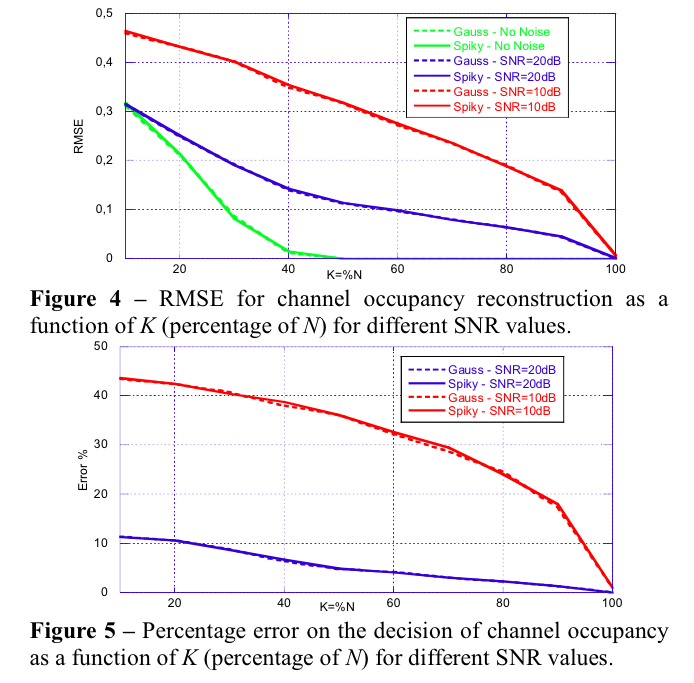
\includegraphics[width=0.75\columnwidth]{figs/cs-cogn-radar.png}
\caption{Block diagrams for mean square error and error detection performance of the proposed compressive cognitive radar systems}
\label{cs-cogn-radar}
\end{figure} 

The experimental results figure \ref{cs-cogn-radar} shows the CS based radar has appealing performance in low sampling rate (using only $ < 30\%$ of the total samples of the original signal) and low detection error in high SNR cases. But in low SNR environment, the proposed system still struggles and suffers. 

\newpage

\section{Further Sensing Task: Hybrid Signal Processing}

\begin{figure}
\centering
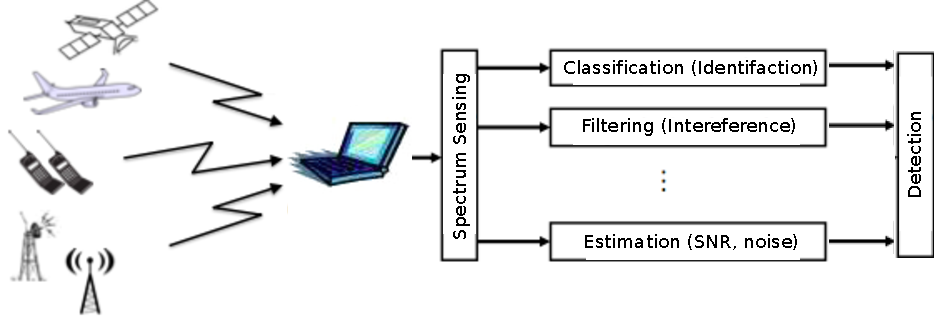
\includegraphics[width=0.75\columnwidth]{figs/hybrid_dsp.pdf}
\caption{Block diagram of hybrid signal sensing, processing and detection in cognitive spectrum sensing}
\label{hybrid_dsp}
\end{figure} 

According to the aim of spectrum sensing that we have talked in section \ref{sct:aim_ss}, the main task is to detect the signal existence of licensed users' (primary users, PUs) from cognitive radio's receivers.

Practically, in order to obtain high accurate detection result, a cognitive radio must keep monitoring almost every useful 'clues' to prove whether a spectrum band is used or not. Such clues (in physical layer) contains various information such as
signal to noise ratio (SNR), modulation mode, primary signal bandwidth, and primary signal power etc. 

As listed, there are too many informations to monitor at cognitive radios' receivers, so most of spectrum sensing algorithm only detect parts of the listed information, some detect power (energy detection), some detect partial signal (matched filtering detection), and others detect cyclic symbols (feature detection). 

As many of those method successfully accomplish the task in different scenarios, such as ED works well in high SNR cases, feature detection performs well in cases where primary signals contains strong periodic information, however, one of the key aims of designing a modern networks, is to make the network flexible enough, where hybrid types of primary signals communications (e.g. TV, mobile phone, radar) are mixed, and time-varying parameters (SNR, noise, power modulation type) based communications are allowed, shown as Figure \ref{hybrid_dsp}. This demand gives rise to a significant uncertainty in signals' appearance, and communication quality. As a result, in most practical cases, hybrid signal communication will co-exist, and for a higher detection results, pre-procedure such as filtering and classification for detection should be considered.

As a result, in cognitive radio, although detection is still a main task, but 
in order to efficiently detect co-existed primary signals, filtering (e.g. interference cancelling),  classification (e.g. hybrid signal separation), and estimation (e.g. SNR prediction) are also needed and regarded as useful auxiliary methods for further complex detection algorithms. 

Therefore, those assistant methods involves many traditional signal processing methods, and how to suitably apply them to process CS sampled data is a big deal because those data are non-linearly sample while traditional DSP algorithms are aiming at linear samples. In this sense, CS reconstruction are
needed, but it is time-consuming.

The problem shows us a further important issue for hybrid signal's processing in CS based cognitive radio, and more details will be introduced as our future research directions in chapter 6. 

\section{Challenges and Discussion}

The compressed sensing based wideband spectrum sensing for cognitive radio provide its outstanding feature in reducing the sampling rate. However, the corresponding drawbacks emerge in real-time ability and energy consumption, mainly due to its computational expensive non-linear reconstruction and energy consuming characters: 

\subsection{Long-Time Feedback Delay}
Accuarcy is cruical for primary detection. Hence, if we applies CS for sampling, the convex optimisation (e.g.basis pursuit) is always needed for data recovery since it provides better accuracy and robustness comparing to greedy methods (chapter \ref{C:compressed_sensing}). However, convex optimisation is time consuming, which cause too long time to fast feed-back. Since feed back is very important for CR, which is responsible to avoid interference and quick reconfiguration, agility and reconfigurablity may reduce.

\subsection{Mismatch for Traditional Signal Processing}
The reconstruction algorithms for CS is non-linear, which indicates that the recovered data are not directly suitable for conventional digital signal processing where traditional recovering only requires cardinal sinc interpolation (linear process). This brings difficulty in directly reuse the traditional method for sensed data.

\subsection{High Energy Cost}
The heavy reconstruction for CS not only brings large time-delay, but also additional energy cost. Compared to linear recovery in traditional approaches, the CS based signal detection additionally required the block for spectrum recovery before further hypothesis detection. 

\section{Conclusion}
Cognitive radio has been widely used and attracting many research attentions in its spectrum sensing techniques. In this chapter, traditional sensing approaches such as energy detection and feature detection are introduced. In order to solve the detection task for wideband and high frequency signals, compressed sensing based spectrum sensing (CS-CSS) is introduced and demonstrated. However, the compressively sampled data does not directly match the traditional processing algorithms.

Then here comes the question: what if we directly perform hypothesis detection without CS reconstruction? If the idea is achievable, the additional energy cost will be eliminated so that the entire energy reduces. Besides, not only detection, if we can expand this idea to filtering, estimation, then more intelligent-based scheme for cognitive radio can be supported in physical layer. The answer refers to our future research aims that shown in the next chapter.

%However, in cognitive radio, most of tasks for spectrum sensing are related to detection, estimation, filtering, classification. This contradiction leads the large additional loss in energy usage and time utilisation when we applies the CS to reduce the sampling limitation in wideband sensing for CR. Then noticing the fully reconstruction is always not needed, we will discuss the future direction in the next chapter, for directly processing compressively sampled data in CR, which aims at extracting effective information without fully recovery so that the entire real-time capability and energy efficiency will be significantly increased. 

%--------------------------------------------------------------------

%This is the common problem termed as cognitive spectrum sensing (CSS), that we face in modern signal processing systems, where the ADCs now use CS framework to solve the problem in high sampling rate. Similarly, CR devices recently apply the CS framework, and successfully achieves low-rate wideband signal acquisition while keeping the sensing accuracy in a high level. 

%--------------------------------------------------------------------
%re-write{
%A fundamental difference between CS and classical sampling is the manner in which the two frameworks deal with signal recovery, i.e., the problem of recovering the signal from the measurements. In the Shannon-Nyquist framework, signal recovery is achieved through sinc interpolation?a linear process that requires little computation and has a simple interpretation. In CS, however, signal recovery is achieved using nonlinear and relatively expensive optimisation-based or iterative algorithms [xx3?5]. Thus, up to this point, most of the CS literature has focused on improving the speed and accuracy of this process [xx6?9].

%However, signal recovery is not actually necessary in many signal processing applications. Very often we are only interested in solving an inference problem (extracting certain information from measurements) or in filtering out information that is not of interest before further processing. While one could always attempt to re- cover the full signal from the compressive measurements and then solve the inference or filtering problem using traditional DSP techniques, this approach is typically suboptimal in terms of both accuracy and efficiency. 

%Our future work takes some initial steps towards a general framework for what we call compressive signal processing (CSP), an alternative approach in which signal processing problems are solved directly in the compressive measurement domain **without** first resorting to a full-scale signal reconstruction.
%}

%--------------------------------------------------------------------
%\section{Cognitive Radio and Spectrum Sensing}\label{sct:cr_and_spectrum_sensing}

%Conventionally, licensed spectrum is allocated in long term and intended to be used only by primary users. However, as the increasing demand for higher data rates for communications, the limitation of the inefficiency usage of licensed spectral resources becomes a great bottleneck. Hence, the idea of opportunistically accessing the unused spectral resources (dynamic spectrum access, DSA) turns to be popular and motivates the develop of cognitive radio (CR). In other words, cognitive radio [2, 3] has become a promising solution to solve the spectrum scarcity problem. 

%For each cognitive radio network, the second users (SUs, unlicensed users) are able to reuse idle spectrum for communications without doing harm to the primary users (PUs, licensed users) when PUs are absent. Further more, cognitive radio can be considered as an developed software-defined radio (SDR) %[Wideband spectrum sensing for cognitive radio networks- a survey]that automatically senses its surrounding environment (e.g. noise level, spectrum usage ,RF stimuli etc) and intelligently adapts its configuration (i.e. operation parameters) to varying network infrastructure, in order to meet the quality of service.

%--------------------------------------------------------------------

%re-write [Wideband spectrum sensing for cognitive radio networks- a survey]
%Cognitive radio is an advanced software-defined radio that automatically detects its surrounding RF stimuli and intelligently adapts its operating parameters to network infrastructure while meeting user demands. Since cognitive radios are considered secondary users for using the licensed spectrum, a crucial requirement of cognitive radio networks is that they must efficiently exploit under-utilised spectrum (referred to as spectral opportunities) without causing harmful interference to the PUs. Furthermore, PUs have no obligation to share and change their operating parameters for sharing spectrum with cognitive radio networks. Hence, cognitive radios should be able to independently detect spectral opportunities without any assistance from PUs; this ability is called spectrum sensing, which is considered one of the most critical components in cognitive radio networks.

%------------

% \subsubsection{X-Digital Signal Processing}
% Recent representative applications for CS signal processing focus on establishing interfaces to link the CS recovered data to the traditional signal processing. One of the popular CS based signal processing architectures is the X-DSP in Xampling\cite{mishali2011xamplingsignal}. This architecture is designed for joint sparse support detection and filtering via the samples from the MWC. The multi-band signal can be presented in quadrature representation:
% \begin{equation}
% \label{eqn_xdsp}
% x(t) = \sum_{i=1}^{N/2} I_i(t) cos(2\pi f_it) + Q_i(t)sin(2\pi f_it)
% \end{equation} 
% , where $I_i (t)$ and $Q_i(t)$ are the real-valued narrow-band signals, and $f_i$ is the unknown carrier frequency. 
% In the former section of modulated wide-band converter, recovering the signal $x(t)$ via MWC is achieved by using the MMV based CS reconstruction. However, since the frequency of the carrier $f_i$ is still unknown, although $z[n]$ in (\ref{eqn_zn}) is recovered, it's not approximate for standard DSP algorithms.
% %The subspace algorithm needs to estimate $f_i$ , $I_i(t)$ and $Q_i(t)$.
% %it is insufficient since the fine recovery of the multi-band signal requires 
% %the information $I(t)$ and $Q(t)$ are not contained in the $z[n]$ in (xa), and the carrier frequency is unknown. Therefore, although z[n] is recovered it's not suitable for standard DSP algorithms.  
% In \cite{mishali2011xamplingsignal}, a refined support detection algorithm, Back-DSP, is proposed by assuming zero cross-correlation between $I_i(t)$ and $Qi(t)$. The Back-DSP algorithm consists of the following steps: %reviseBegin
% 
% 1. Refining the coarse support estimate $f_i$ to the actual band edges using prior information of the minimal width of a single band and the smallest spacing between bands.
% 2. Obtain a sequence $s_i[n]$ for each $1 ≤ i ≤ N/2$, such that $s_i[n]$ contains the entire contribution of exactly one band.
% 3. Estimating $f_i$ using a digital version of the balanced quadricorrelator(BQ) from $s_i[n]$. The information signals $I_i(t)$ and $Q_i(t)$ are obtained based on $f_i$.
% 
% With Back-DSP, we can now reconstruct x(t) using \ref{eqn_xdsp}, which requires only N mixers, filters and DACs. In addition, note that once the information signals $I_i(t)$, $Q_i(t)$ are obtained, error correction DSP algorithms can be employed to improve the overall robustness to noise. %reviseEnd

% %------------------------------------------------------
% 
% \subsection{Hypothesis Test}
% 
% The aim of spectrum sensing is to decide whether a particular sub-band of the spectrum is available or not. In other words, the procedure is to discriminate based on two hypotheses in equation \ref{detect_hypo}: 
% \begin{equation}
% \label{detect_hypo}
% \begin{aligned}
% Hypothesis0 (H0): y[n] = w[n], \quad n = 1,..., N   \\
% Hypothesis1 (H1): y[n] = w[n] + x[n] , \quad n = 1,..., N
% \end{aligned}
% \end{equation}
% , where $x[n]$ is the primary user's signal, $y[n]$ is the vectorial observation, $w[n]$ is the noise, and $n$ refers to time slots. The hypothesis 1 suggests that the primary user's signal exists, while hypothesis 0 suggests no. Typically, the decision is made by comparing a predetermined threshold with test statistic $\Lambda(y)$ in equation \ref{detect_hypo}: 
% \begin{equation}
% \label{detect_hypo}
% \Lambda(y) \mathop{\lessgtr}_{H_1}^{H_0} \alpha
% \end{equation}
% Then the performance of a detector is quantified by the receiver operating characteristics (ROC) curve, which presents the probability of detection $P_D = Prob(\Lambda(y) > \alpha, H1)$ and false alarm probability $P_fa = Prob(\Lambda(y) > \alpha, H0)$. 
% 
% 
% %------------------------------------------------------
% 
% \begin{itemize}
%   \item \textbf{matched filtering \cite{poor1994introduction}} In the case where the signal $x$ to be detected is perfectly known (i.e. mean and variance), then the observation $y ~ N(x, \delta^2 I)$ under $H1$, and the optimal test statistic of the matched filter becomes: 
% \begin{equation}\label{match-filter}
% \Lambda(y) = Re[x^H y] \mathop{\lessgtr}_{H_0}^{H_1} \alpha
% \end{equation}  
% However, in practice the signal and noise parameters are not always known to the system, and its required carrier synchronization is difficult to implement. The hardware architect is shown in figure \ref{narr_spec_sens}.a.
%   \item \textbf{energy detection \cite{urkowitz1967energy}} 
% In many cases, the signal to be detected does not present enough structure information, then energy detector produces the optimal choice of detection by choosing the test statistic $\Lambda(y)$ as 
% \begin{equation}
% \Lambda(y) = \frac{y^2}{\delta} \mathop{\lessgtr}_{H_0}^{H_1} \alpha
% \end{equation}
% The implementation are of energy detector is simple shown in \ref{narr_spec_sens}.b. However, it cannot distinguish the different primary users signals, and provides poor detection performance in low SNR scenarios. 
%   \item \textbf{feature detection} cyclostationary feature detection \cite{enserink1994cyclostationary} detects and discriminate between different types of primary signals by exploiting their cyclic non-stationary features. For instance, the orthogonal frequency-division multiplexing (OFDM) signal have a explicit correlation structure due to the cyclic prefix (CP) between transmitted data at the transmitter. The architecture of this detector is presented in \ref{narr_spec_sens}.c. However, the computational cost is relatively high.
% \end{itemize}
% 

%----------------compressed sens vs filter-bank------------

%In such case, if weconvert the signals for lower rate sampling, the analog filter-bank must be very complex design with heavy cost, for instance, large filter bank which covers the whole bandwidth, or adaptive filter but cost long time frequency shifting. If we intend to reduce the design complexity and cost, however, the sampling rate should be relatively high with less filters for down-conversion. 

%----hypothesis model----
% The aim of spectrum sensing is to decide whether a particular sub-band of the spectrum is available or not. In other words, the procedure is to discriminate based on two hypotheses:
% \begin{equation}
% H0: y = w \quad (noise case)
% H1: y = w + x \quad (primary signal case)
% \end{equation}
% , where $x$ is the primary user's signal, $y$ is the vectorial observation, $w$ is the noise, and $n$ refers to time slots. Typically, the decision is made by comparing a predetermined threshold with test statistic $\Lambda(y)$ ideally defined by the likelihood ratio. The performance of a detector is quantified by the receiver operating characteristics (ROC) curve, which presents the probability of detection $P_D$ and false alarm probability $P_fa$. 
% \begin{equation}
% P_D = Prob(\Lambda(y) > \alpha, H1)
% P_fa = Prob(\Lambda(y) > \alpha, H0)
% \end{equation} 
